% 
%  chapter2.tex
%  ThesisISEL
%  
%  Created by Matilde Pós-de-Mina Pato on 2012/10/09.
%
\chapter{State of the Art}
\label{cha:users_manual}

Firstly, on section \ref{sec:related_work}, will be made an overview on previously developted work made on this subject, then, on section \ref{sec:async_concepts}, will be made a characterization of the key concepts related to it. By last, on section \ref{sec:state_of_the_art}, are presented and explained several technologies representative of the state of the Art on asynchronous data flow in different programming realities, e.g. on Kotlin, JAVA and C\#. 


% ================
% = Related work =
% ================
\section{Background} % (fold)
\label{sec:related_work}

% Initially, when computers had a single processing unit, the networks only allowed the exchange of few bytes per second and the data servers didn't had the responsiveness requirements that are mandatory today; software computational systems were simpler, in the sense that operations were mostly made in a single execution thread. 
% The servers design, were made without many concerns about availability under demand pressure or computer resource optimization. 
% Consequently, operations that required intensive IO interactions or data request from an external sources, were mostly blocking, non-flexible in terms of responsiveness and interoperability. 

From the end of 80´s to the beginning of the 2000´s, with the acceleration of Moores´s Law in hardware and network bandwidth development, the creation of the web as we know today through the wide spread of use of the HTTP protocol and the support from new operative systems to multithreading support, the necessity of high responsiveness servers started to grow. This increase in demand of new ways to handle data through parallelism, caused the necessity of design new programming models compatible with concurrent work. 

Taking the wave initiated by the Gang of Four in \cite{gof}, where 23 patterns were compiled to deal with object-oriented problems, a group of researchers published the \textit{Proactor Pattern} in the paper \cite{proactor} to deal with asynchronous IO. 
In the document, are identified four properties that high-performance web server must have: 
\begin{itemize}
	\item Concurrency - The server must process multiple client requests simultaneously.\\
	\item Efficiency - The software design must be built aiming the use of least hardware resources as possible. \\
	\item Simplicity - The code of the solution must be easy to understand, modular and avoid own built design patterns as possible. \\
    \item Adaptability - The system must be totally decoupled from client implementations, allowing it to be easily used by any client independently of the underlying technologic realities. To achieve this, may be used standards e.g. \cite{REST} or SOAP.\\
\end{itemize}

The authors propose the \textit{Proactor Pattern}, because in their opinion, conventional concurrency models fail to fully achieve the enumerated properties. In the paper, before presenting the \textit{Proactor Pattern}, are identified two major concurrency models, namely: \textit{multithreading} and \textit{reactive event dispatching}. 

The paper refers that one of the most direct implementations of the multithreading approach, is the handling of multiple requests by creating a new thread every request. Each request will then be fully processed and the recently  created thread is then be disposed after the work is finished. 

This solution has several serious issues. Firstly, creating a new thread per request is highly costly in terms of computational resources,
because are involved context switches between user and kernel modes; secondly, must be taken in account synchronization to maintain data integrity.
Then, the authors warn about the fact that the IO retrieved data is mainly memory-mappped, wich rises the question: What happens when the data obtained through IO becomes greater than the system memory can hold? The system stalls until more memory becomes available!?
On last, if the server receives a high demand of requests, the server easily blocks in the process of creating and disposing threads. 

To avoid this issue, the authors, recommended the use of dynamic threadpools to process requests, where each request will be linked to a pre-existing thread, avoiding all the overhead of creating and disposing a thread per request;
however, issues related with memory-mapping and overhead due to the switching of data between different threads maintains. 

Another traditional concurrency model identified by the authors of the paper, is the \textit{Reactive Synchronous Event Dispatching} or more commonly known as \texttt{Reactor Pattern}. In this model, a \textit{Dispatcher}, with a single thread in a loop, is constantly listening requests from clients and sending work requests to an entity named \textit{Handler}. 
The \textit{Handler}, will then process the IO work Synchronously and request a connection to the client in the \textit{Dispatcher}. When the requested connection is ready to be used, the \textit{Dispatcher} notifies the \textit{Handler}. After the notification, the \textit{Handler} asynchronously sends the data, that is being or has been obtained through IO, to the client.\\
Although the authors identifying that this approach is positive, because decouples the application logic from the dispatching mechanisms besided with the low overhead due the use of a single thread, the authors identify several drawbacks with this approach. 
Firstly, since IO operation are synchronous, the code for this approach is complex because must be set in place mechanisms to avoid IO blocking through hand off mechanisms. 
Then, if a request processing blocks, the processing of another requests may be impacted. 

To keep the positive points but mitigating the identified issues of previous approaches, is suggested the \textit{Proactor Pattern}. 
This pattern is very similar to the \textit{Reactive Synchronous Event Dispatching}, however, after the requests processed by a single threaded \textit{Completion dispatcher}, 
the IO work is then dispatched asynchronously to the underlying OS IO subsystems, where multiple requests can be processed simultaneously. 
For the result to be retrieved, is previously registered a callback in the \textit{Completion Dispatcher} and the OS has the responsibility to queue the finished result in a well known place. 

Finally, the \textit{Completion Dispatcher} has the responsibility to dequeue the result placed by the OS and call the correct previously registered callback. 
With this, this model creates a platform that provides: decoupling between application and processing mechanisms,
offers concurrent work without the issues inherent with the use of threading mechanisms and since IO is managed by the OS subsystems, is avoided code complexity in handling possible blocking and scheduling issues.  

The \textit{Proactor Pattern}, creates the ground for several models used by modern platforms that use a single/few threads to process client requests and parallel mechanisms to do the heavy work in the background; namely, for example: \textit{Javascript NODE.JS}, \textit{Spring Webflux}, \textit{vertx} and others.

From what was explained until now, is evident the tendency followed by software architects in terms of asynchronous processing from non-reactive to event driven approaches. Initially the systems were non-reactive, where each request had to be processed in a 
specific thread and that thread blocked until something got ready to go further. 
Then, with the asynchronous systems based on events with the introduction of callback systems inspired in patterns like the \textit{Reactor} or \textit{Proactor}; the software design started to become more event driven, allowing the servers to be more efficient in responsiveness, flexibility and resources optimization. 

However, are some limitations in these asynchronous models. For example, if the data to be processed is bigger than the memory available or if the data to be calculated is from a source that produces data at a constant rate that must be processed in real time, these models work badly.  
The traditional models fail to comply these objectives because are mostly eager by design or not comply with the notion of a continuous source of information that requires to be processed in real time.
Taken this in account, projects like project Reactor, Asynchronous Enumerable provided by Microsoft or papers like \cite{LAZYVSEAGER}, try to deal with these issues, by providing API's that merge the concepts of Fluent API's, functional programming and code syntax that tries to resemble synchronous code, being the complexity inherent with asynchronous models implementations hidden from the programmer. 

\clearpage
%\begin{figure}[ht]
%	\centering
%	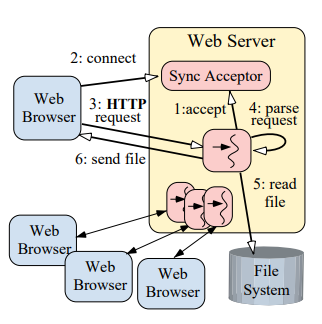
\includegraphics[width=0.65\textwidth]{alternative_1}
%	  \caption{Multithreading solution example}
 % \label{fig:bibtex}
%\end{figure}


%\begin{figure}[ht]
%	\centering
	%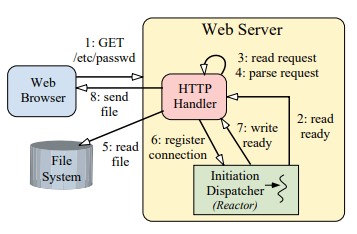
\includegraphics[width=0.65\textwidth]{alternative_2}
%	  \caption{Dispatcher example}proactor
 % \label{fig:bibtex}
%\end{figure}

%\begin{figure}[ht]
%	\centering
%	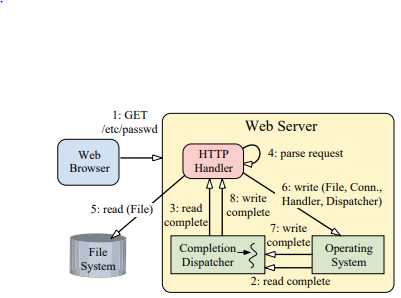
\includegraphics[width=0.65\textwidth]{alternative_3}
%	  \caption{Proactor example}
%  \label{fig:bibtex}
%\end{figure} %

% section introduction (end)

% ====================
% = Folder Structure =
% ====================
\section{Asynchronous flow key concepts and design alternatives} % (fold)
\label{sec:async_concepts}

With the development of several approaches related to asynchronous data flow in several programming plataforms; a dictionary
of properties, concepts and design alternatives started to grow by itself. In the following, are discussed several of the concepts related with asynchronous data flow, namely:

\subsection{Synchronous versus Asynchronous}
	Before explaining more terms related with asynchronous data flow, it's important to clarify what is synchronous and asynchronous in programming. 
	
	Asynchronous in programming, is a call to a function or routine that returns immediately, not blocking the caller until the operation is finished. The operation processing, will be completely independent from the caller execution process and can even be done in another machine. This way, the caller is freed to do more work, even to start \texttt{N} more operations in parallel. 
	
	Meanwhile, a call to a synchronous function or routine, blocks the caller until the operation finishes. In this case, the caller has to wait for the completion of the synchronous operation before going forward, which limits the program efficiency if parallelism is applicable.
	To better visualize what was explained, we have the following examples: 
	
	\begin{figure}[H]
		\centering
		\begin{subfigure}[h]{1.2\textwidth}
			\centering
			\lstfromfile{java}{1-14}{Asynchronous call example}{async}{showlines=true,morekeywords={begin,System,out,print},numbers=left, firstnumber=1}{async.java}
			\label{fig:ra-vectorial}
		 \end{subfigure}	
	\qquad
		 \begin{subfigure}[h]{1.2\textwidth}
			\centering
			\lstfromfile{java}{1-15}{Synchronous call example}{Sync}{showlines=true,morekeywords={begin,System,out,print},numbers=left, firstnumber=1}{Sync.java}
			\label{fig:ra-raster}
		\end{subfigure}		
	  \caption{Example of Synchronous and Asynchronous calls in JAVA}
	  \label{fig:figura-completa}
	\end{figure}
	
	As we can see, in the synchronous call example, the operation return only happens after the whole subsequent remote operation is finished, consequently, the caller operation is dependent from several variables to go forward e.g. : HTTP messaging latency, remote server operation speed or bandwidth issues. 
	Meanwhile, in the asynchronous operation call, the return happens immediately after the call, however, the processing inherent with that operation will start just when the subsystem that handles the asynchronous function is ready to process that work, for example, when the OS is ready to process the received responses from a remote server that handled the operation.

	\subsection{Push vs Pull}
	Another concept important to understand how asynchronous data flow is handled in programming, is the \textit{Pull} and \textit{Push} processing patterns.
	In \textit{Pull} pattern, usually, exists a source of data and the program iterates over that source to operate over each item. 
	
	On the other hand, in the \textit{Push} pattern, the items of the data source are "Pushed" to a routine that will operate over that item.
	To help to assimilate what was just explained, we have the following example:

	\begin{figure}[H]
		\centering
		\begin{subfigure}[h]{1.2\textwidth}
			\centering
			\lstfromfile{java}{1-17}{Pull pattern example}{pull}{showlines=true,morekeywords={begin,System,out,print},numbers=left, firstnumber=1}{pull.java}
		 \end{subfigure}	
		 \begin{subfigure}[h]{1.2\textwidth}
			\centering
			\lstfromfile{java}{1-17}{Push pattern example}{push}{showlines=true,morekeywords={begin,System,out,print},numbers=left, firstnumber=1}{push.java}
		\end{subfigure}		
	  \caption{Example of Pull and Push data handling patterns}
	  \label{fig:exmplo2}
	\end{figure}
	\clearpage

	As we can see, in the pull pattern, the items are "pulled" from a data source through an iteration mechanism. 
	
	In contrast with that, in the \textit{Push} pattern, items are pushed to a consumer through a supplier.


	\subsection{Hot versus Cold}
	
	Another property that must be took in account when handling with \textit{Reactive Streams} or asynchronous data processing in general, is the nature of the data flow. 
	There are two main adjectives to name a data flow, \texttt{Hot} or \texttt{Cold}. 

	A \texttt{Cold} data flow, is a flow of information that is produced just when the stream pipeline in subscribed by an observer. In this case, the producer only starts sending/producing data when someone is interested in the data from that source. 
	For example, when program uses a IO mechanism to lazily retrieve a sequence of words from a database, the IO mechanism will only start sending information just when a consumer subscribes that data flow. Usually, the data is sent to the consumer in unicast.
	
	On the other hand, in a \texttt{Hot} data flow, the data is produced independently of existing any observer to that information. This mechanism usually work in broadcast and the data is continuously produced and sent to possible observers.
	In this case, when an observer subscribes to a publisher, exists the possibility of data items being already lost to that publisher while in the \texttt{Cold} flow, the consumer usually receives all items that were produced by the source.
	In the following examples, a number is produced each 100 milliseconds:

	\begin{figure}[H]
		\centering
		\begin{subfigure}[h]{1.2\textwidth}
			\centering
			\lstfromfile{java}{1-3}{Cold Example}{cold}{showlines=true,morekeywords={begin,System,out,print},numbers=left, firstnumber=1}{ColdFlux.java}
		 \end{subfigure}	
	\qquad\qquad
		 \begin{subfigure}[h]{1.2\textwidth}
			\centering
			\lstfromfile{java}{1-6}{Hot Example}{hot}{showlines=true,morekeywords={begin,System,out,print},numbers=left, firstnumber=1}{HotFlux.java}
		\end{subfigure}		
	  \caption{Example of Hot and Cold data streams}
	  \label{fig:exmplo3}
	\end{figure}

	
	As we can see, in the \texttt{Hot} data flow example, the items are emitted from the moment the producer is created, independently of existing any subscriber or observer attached to that publisher. Notice that when a consumer is subscribed to the publisher, 1 seconds after the emittion started, the numbers from 0 to 10 were not printed.
	
	In the \texttt{Cold} example, the producer only emits data when a subscription is done, and because of that, all the produced numbers were printed, in contrast with what happen in \texttt{Hot} stream, where data loss are almost certain. 
	\clearpage
	\subsection{Cancelables} 
	As already stated above, Asynchronous operations may run outside the main program context. 
	This implies, that the main program loses visibility and control on what happens in that asynchronous operations.
	Because of that, exists the need to put in place mechanisms of control that allow the main program to maintain control over an asynchronous operation to, for example, cancel the operation or put in place finishing logic that allow, for example: resource disposing, logging, decisions etc...

	These mechanisms, are many times done through the concept of \textit{cancelables}. 
	Usually, a cancelable, is an entity that represents an operation that can canceled from an external entity, or, an entity that allows to set logic when an operation finishes by any reason.
 
	In C\#, a cancelable is an interface implemented by objects that represent asynchronous operations and provides the means to cancel asynchronous operations, on the fly. 
	This is achieved through a mechanism named: \texttt{CancellationToken}, that is used to pass information through different execution threads. 
	
	In RXJava, a \texttt{Cancelable}, is a functional interface with the method \texttt{cancel()}. Then, the \texttt{Cancelable} can be associated to a data source representation, the \texttt{Observable}, by calling the method \texttt{Observable.setCancelable(Cancelable)}. 
	When the \texttt{Observable} finishes or is canceled for any reason, the method \texttt{Cancelable.cancel()} will be called. 
	This way,  proper logic is put in place to handle an asynchronous operation cancelation.
	
	As we saw, these two concepts of cancelable diverge. One, provides the means to cancel an operation on the fly and gives some control over the operation cancelation; the other, provides the means to control an operation cancelation independently of how it was cancelled.
	
	\clearpage
	\subsection{Error Handling}  
	In synchronous environments, usually, when something goes wrong, the way to handle an error in the majority of cases its by throwing an exception and propagate it until the proper code handles it, usually  in a try/catch block. 
	However, in cases when exists an asynchronous operation or when a continuous stream of data items are being received, that way of dealing with an error can imply several issues, e.g: exceptions not reaching main program, log losing or asynchronous flow blockage. 
	
	Since log losing or blocking a whole operation because of a badly handled error is unacceptable, the best way to deal with errors in asynchronous data flow it is to isolate the error. This way, the flow processing may continue in parallel while the error is properly handled.
	
	The best way to handle this kind of errors, it is to have proper callbacks that are called when an error occurs on the stream item. This way, a function can handle the error properly, without the necessity to blocking any data stream processing, if avoidable and the proper logging and any additional measure to handle it can be put in place.
	\clearpage
	

	\subsection{Intrisic Keywords} 
	
	Asynchronous code is tendentiously harder to understand because, in opposition with what happens in synchronous code, the sequence of programming statements operations may not happen chronologically ordered. 
	Because of that, many times it's difficult to debug and sustain asynchronous code. 

	For that reason, many languages started to add syntax techniques that allow the programmer to build asynchronous code that resembles the synchronous syntax.
	Under the hoods, the virtual machines that sustain these syntax mechanisms, handle the code bounded with that 'intrisic words'and builds asynchronous routines that the programmer will not be aware of;
	being this a way to abstract the programmer from the complexity of handling and sustaining complex asynchronous code. 

	One example of \textit{intrinsic words} mechanisms, is the \texttt{async...await} keywords implemented in \textit{Microsoft's .NET C\#} and in \textit{javascript}. 
	
	In the example \ref{fig:enumex} we can see an example of these keywords being used. 
	Where, for example, we can observe in the line 15, a call to a asynchronous operation, and, by hadding the keyworkd \texttt{await}, the next statment although being to an asynchronous operation the statment orde looks like its synchronous. 
	
	Another example of 'intrisic words' used in asynchronous processing is the \texttt{for await...of}, used in javascript to proccess asynchronous enumerables. 
	

	On the sub chapters of \ref{sec:state_of_the_art} these examples will be explained with more depth.
	\clearpage

	\subsection{Back-pressure} 

	When the \textit{pull} method is used to retrieve items from a source, the producer retrieves only the items it can process in the given time. 
	
	However, when the \textit{push} approach is used as data retrieval method from asynchronous flows, the producers have the initiative to push items to its consumers. 
	This can originate situations, where the producer emits items faster than the producers can handle, which can create problems like: unwanted loss of data, lack of responsiveness from consumers, etc... 
	
	To resolve these issues, were created strategies and design patterns that are commonly referred as \textit{Backpressure}.
	There are four main approaches which the majority of \textit{Backpressure} strategies are designed from and can be resumed as: 
	
	\begin{enumerate}
		\item \textbf{DROP:} Producer drops items after a retrieving buffer gets full.
		\item \textbf{Buffer everything:} A buffer, keeps all unprocessed items that are received. Usually, this strategy is used when all received items are critical for the business development and memory managment has flexibility to handle the increase of storage needs.
		\item \textbf{Error:} An error is thrown when the buffer threshhold is reached, usally all items received after the threshhold is reached are discarded.
		\item \textbf{Lastest:} Only the last received item in the given moment is kept.
		\item \textbf{Missing:} No back-pressure strategy it is in place, all items that ca not be processed on arrival, are discarded.
	\end{enumerate}
	\clearpage
% The template file for writing dissertations in  \texttt{LaTeX} is organized into a main directory, a set of files and sub-directories:
% \begin{enumerate}
% 	\item[ThesisISEL] This is the main directory and includes:
% 	\begin{enumerate}
% 		\item \textbf{Logo} Directory with Faculty logos;
% 		\item \textbf{sty} Directory will all sty files that help in formatting document;
% 		\item \textbf{Chapters} Directory where to put user files (text and figures);
% 		\begin{enumerate}
% 		\item \textbf{scripts} Directory with useful bash scripts, e.g., for cleaning all temporary files;
% 		\item \textbf{img} Directory with all images of your thesis;
% 		\end{enumerate}
% 		\item \textbf{alpha-pt.bst} A file with bibliography names in portuguese, e.g., 'Relatório Técnico' e 'Tese de Mestrado' instead of 'Technical Report' and 'Master Thesis'. This file is used automatically if Portuguese is selected as the main language (see below);
% 		\item \textbf{defaults.tex} A file with the main default values for the package (institution name, faculty's logo, degree name and similars);
% 		\item \textbf{personaldataofthesis.tex} A file with the main default values for the package (identification of report as well as the author and juries);
% 		\item \textbf{template.tex} The main file. You should run  \texttt{LaTeX} in this one. Please refrain from changing the file content outside of the well defined area;
% 		\item \textbf{bibliography.bib} The bib file. An easy way to find to import citation into \texttt{bibtex} is select option \texttt{Show links to import citation into
% Bib\-Tex} in \href{http://scholar.google.pt/scholar_settings?hl=en&as_sdt=0,5}{\texttt{Scholar google settings}}.
% 		\item \textbf{thesisisel.cls} The  \texttt{LaTeX} class file for the thesis{} style. Currently, some of the defaults are stored here instead of \verb!defaults.tex!. This file should not be changed, unless you're ready to play with fire! :)
% 	\end{enumerate}
% \end{enumerate}

% Again, we would like to recall that all the user \texttt{LaTeX} files should be stored in the \verb!ThesisISEL! directory, and all the images in \verb!ThesisISEL/Chapters/img! directory.\todo[inline]{Yet another note!}
% section folder_structure (end)

% ===================
% = Package options =
% ===================
\section{State of the Art} % (fold)
\label{sec:state_of_the_art}

In this section, we will be explaining the different frameworks that are the \textit{State of the Art} in asynchronous data processing in several programming languages.

First of all, in the section \ref{reactivex}, will be presented the multi-language \texttt{reactivex.io} project, and how the \texttt{Observer Pattern} is used in this project to implement real time asynchronous processing with and without \textit{back-pressure}.

Secondly, in the section 2.3.2, will be presented the \textit{.NET} \textit{Async Enumerables} and how this approach diverges from approaches made in \textit{reactivex.io}, \textit{Javascript}, and in Kotlin with \textit{Kotlin Flow}.
In the sections 2.3.3 and 2.3.4, will be respectively presented the Javascript and the Kotlin Flow strategies for asynchronous data processing.

Finally, in the section 2.3.5, will be made an overview and taken conclusions about the different technologies presented, and how each approach can be used for different problems and objectives. Then, will be made a theoretical prediction on how each technology behaves in several know circumstances. 

\subsection{ReactiveX.io Project}
\label{reactivex}

After the historical context explained in the chapter 2.1, many groups of developers started to implement several solutions to handle asynchronous data flows. One of the most ambitious results of this proactivity is the \textit{reactiveX} project.

This project gathers several ideas and known design patterns to implement an asynchronous data flow mechanism. 
The most positive points about this project implementation is that the mechanism is implemented in several programming languages using an open source approach and the solution design is done in a way, that all the complexity inherent with asynchronous programming is hidden from the programmer, making the code very intuitive and iterative an easily understandable for programmer that are not used to handle with asynchronous enviroments. 
In this dissertation, we will analyze the implementation of reactiveX made for Java, which is named: RXJava
\clearpage
\subsubsection{RxJava architecture}
\label{rxjava}
To implement an asynchronous mechanism that can handle \texttt{Hot} and \texttt{Cold} data flows with and without back-pressure, the project adopted the \textit{Observer pattern} allied with the concepts described in the \textit{Publishes/subscriber pattern}.
The designers justify this choice by saying that this model allows treating streams of asynchronous events with the same simplicity made in the synchronous counterparts e.g. in \texttt{Collection} and \texttt{Iterator}. The designer complement the justification by saying that, using this approach, the code complexity inherent with low-level threading, non-blocking IO, thread-safety etc... are completely abstracted from the programmer.

In the implementation, the data source/publisher of an asynchronous stream of events is represented by the classes \texttt{Observable} and \texttt{Flowable}. In this case, the only difference between \texttt{Observable} and \texttt{Flowable}, is that the class \texttt{Flowable} supports back-pressure through different bufferization strategies.

On a side note, it is important to refer that in RxJava, the same way \texttt{Observable} and \texttt{Flowable} represent a stream of N events, exists a single event is represented by a class named \texttt{Single}.

One of the great advantages of using this framework, is that the \texttt{Observable} and \texttt{Flowable}, although representing asynchronous data source, offer fluent API's that allows chaining operation fluently, like it is done in e.g, on java \texttt{Stream} implementation.
In these fluent API's, stream processing operations like: \texttt{filter}, \texttt{flatMap} or \texttt{distinct} are available, allowing to treat these asycnhronous sequence of items like is made with synchronous streams.

On the other hand, the observers/subscribers are represented by consumers that are attached to \texttt{Observable} through the method \texttt{Observable.subscribe()}.
The consumers can be either implementations of the functional interface \texttt{Consumer<T>} or implementations of the interface \texttt{Observer}.

The \texttt{Observer} interface is built with the intent to offer an extra control over the stream processing through error handling, which a \texttt{Consumer<T>} implementation lacks. The \texttt{Observer} can be viewed as the asynchronous representation of the java util interface \texttt{Iterator}, the resemblance can be seen by seeing the interface \texttt{Observer} methods:

\begin{enumerate}
     \item \texttt{onSubscription()}: Method called right after the subscription is made with an \texttt{Observable} 
	 \item \texttt{onNext(T item)}: Method called when an item is emmitted by the asynchronous data source.
	 \item \texttt{onError()}: In contrast with Iterator, the RxJava \texttt{Observer} is equipped to support error handling. This callback will be called when an error occurs.
	 \item \texttt{onComplete()}: Method called when the data source closes or if the subscription finishes.
\end{enumerate}	

Since its possible to make a relation between synchronous and its asynchronous logic counterparts in many languages, on next, we will take as example the relation between \texttt{Java} library and how these objects can be directly related to their asynchronous counterparts in \texttt{RXJava}.
On the next table, it is possible to see how each object type can be mapped 

\begin{center}
\begin{tabular}{ |l|c|c| }
\hline
	& Single Item & Multiple Items \\ \hline
	Java & & \\ 
& \texttt{T getData()}  & \texttt{Iterable<T> getData()} \\
	& & \\
	\hline
	RxJava & & \\ 
& \texttt{Single<T> getData()} & \texttt{Observable<T> getData()} \\
	& & \\
	\hline
\end{tabular}
\end{center}


\subsection{Asynchronous Enumerables}
	\label{sec:aenums}
	To better understand what an asynchronous enumerable is, firstly, we must define what Enumerables are. 
	
	An enumerable, is the logical representation of a collection that can be iterated. 
	In synchronous programming, this is usually made by creating a Collection class, that implements a mechanism that enables iteration over its items.
	
	On the other side, in the asynchronous world, many times exists situations where a stream of data items are constantly arriving from a remote source, the commonly named \textit{asynchronous Flows} or \textit{asynchronous streams}. 
	
	The software designers saw, that did not exist many logical differences between a collection and real time data sources; 
	the only difference was that a collection items could be retrieved on demand from memory, while the data flows are iterated over time when items become available for consumption.

	Taking all this in account, has born the idea of creating the notion of the asynchronous enumerable, where the asynchronous enumerable is the representation of a constant source of readable items.
	With the use of this concept, were implemented several mechanisms, e.g. the AsyncEnumerables in C\#, that simplify the iteration over asynchronous data sources. 
	Making the code similar to synchronous statements, easier to maintain, and, once again, abstracting the programmer from many complex details inherent with asynchronous processing.

\subsubsection{.NET Asynchronous Enumerables}
\label{csenums}
	\texttt{IEnumerable<T>} in C\#, is a interface that implements a method \texttt{GetEnumerator()} that returns a \texttt{IEnumerator<T>}. 
	In its turn, \texttt{IEnumerator<T>}, is a interface that allows to iterate over items of a Collection by offering a method \texttt{T getCurrent()}, that allows to retrieve the current item 
	and a method \texttt{bool MoveNext()}, that allows to iterate to the next item of the sequence and check if the iteration has finished.
	\texttt{IAsyncEnumerable<T>}, keeps the same logic of \texttt{IEnumerable<T>}, but instead of returning a synchronous \texttt{IEnumerator<T>} with a synchronous \texttt{MoveNext()} method, returns a \texttt{IAsyncEnumerator<T>} where its method \texttt{bool MoveNextAsync()} is asynchronous. 
	
	On the other side, the keyword \texttt{yield}, is a syntax sugar introduced in \textbf{C\# 2.0} that allows to avoid the implementation of \texttt{IEnumerable<T>} and \texttt{IEnumerator<T>} interfaces by the programmer,
	allowing iteration and the lazy return of items. All the work of implementing iteration interfaces is handled by \texttt{.NET} virtual machine in background. 
	On top of that, the use of \texttt{yield} is compatible with asynchronous iteration involving \texttt{IAsyncEnumerable<T>}, which simplifies interation of asynchronous flows in C\#, as we can see in the next example:
	
	\begin{figure}[H]
		\centering
		\lstfromfile{java}{1-33}{}{asyncenumerables}{showlines=true,morekeywords={begin,Console,async,await,static,for, yield},numbers=left, firstnumber=1}{asyncEnum.cs}
		\caption{C\# Asynchronous Enumerables example}
		\label{fig:enumex}
	\end{figure}

\subsubsection{Javascript asynchronous iterables}
\label{jsae}
	Javascript tries to provide a functional and weakly typed approach to asynchronous flow processing, opposed to what we saw in the C\# solution.

	The keyworkd to provide the mechanism to iterate over asynchronous streams in relativity similar to what we saw in C\#, with the implementation of the intrisic keywords \texttt{async...await} and \texttt{for await...of}.

	With the keyword pair \texttt{async...await}, its provided the syntax "sugar" that enables to make asynchronous calls and the code syntax resembling synchronous. 
	The \texttt{async} mark is used in an asynchronous function and enables the use of the keyword \texttt{await}. The \texttt{await} keyword is then used in an asynchronous call to another asynchronous function

	On the other side, the keywords \texttt{for await...of}, provides support for iteration over asynchronous enumerables, as we can see in the next example:

	\begin{figure}[H]
		\centering
		\lstfromfile{java}{1-30}{}{asyncenumerables}{showlines=true,morekeywords={begin,Console,async,await,static,for, of},numbers=left, firstnumber=1}{asyncenum.js}
		\caption{Mozilla's Javascript Asynchronous Enumerables example}
		\label{fig:enumex2}
	\end{figure}

In this example, the function \texttt{streamAsyncIterable} read a stream of bytes and has the responsibility to lazily return the items as they become available.

On the other side, the function \texttt{getResponseSize}, the keyword \texttt{await} its followed by an asynchronous HTTP request and the mechanism \texttt{for wait...of} it is used to iterate over an asynchronous iterable stream. As we can observe, the code syntax is very similar to a synchronous iteration. 

With the implementation of this mechanism, javascript simplifies in a very subtle way, how asynchronous streams are handled, allowing the code to be easily readable and maintainable and abstracting the programming from: e.g. callbacks, tasks or completion tokens.

This solution is usually used in front-end environments, for example, to load several items from remote sources while a web page loads.

\subsection{Kotlin Flow}

Kotlin asynchronous flow implementation is a \ref{Reactive Streams} compliant solution and similarly to RxJava, Kotlin strongly typifies a stream of N events, which, in this case, is done through the implementation of the interface \texttt{Flow<T>}.
The \texttt{Flow<T>} implementation is done through a builder, like we can see in the next example:

\clearpage
	\begin{figure}[H]
		\centering
		\lstfromfile{java}{1-6}{}{kotlinflow}{showlines=true,morekeywords={fun,Flow<T>,suspend,emit,static,for, of},numbers=left, firstnumber=1}{flow.kt}
		\caption{Flow builder}
		\label{fig:kotlinflow}
	\end{figure}
\clearpage

To start listening a particular data stream is mandatory to the subscriber to call the method \texttt{Flow.collect()} that starts the emission of items of a cold flow.
On the other side, to represent Hot flows, must be used the used the interface \texttt{SharedFlow<out T> : Flow<T>}. 

The main difference between the kotlin implementation on these two interfaces, is at the result of \texttt{collect()} call. 
While the \texttt{Flow.collect()}, because of its cold nature, starts the flow everytime its called, resulting in the limited emission of the same set of items; the \texttt{SharedFlow.collect()} emission of events never finishes.
On the other side, while the \texttt{Flow.collect()} call context is private to the caller, the \texttt{ShareFlow.collect()} is shareable by N subscribers, which makes this solution ideal for broadcast mechanisms.

To start listening the stream of events is callent the betword

\clearpage
	\begin{figure}[H]
		\centering
		\lstfromfile{java}{1-24}{}{kotlinflowcold}{showlines=true,morekeywords={fun,Flow<T>,suspend,emit,static,for, of},numbers=left, firstnumber=1}{flowcold.kt}
		\caption{Kotlin flow example}
		\label{fig:kotlinflowcold}
	\end{figure}
\clearpage


Likewise RxJava, \texttt{Flow<T>} provides a fluent API of intermediate operators that allow item processing, through the traditional upstream processing push methods, like: filter, map, zip,take etc...   . On the othe se executed recurring to different execution contexts, for exemple, to change the running thread from the main programm to a custom thread scheduler.




Relatively to the use of intrisic words, Kotlin offer the \texttt{suspension} key word that as the same  

uses the function \texttt{emit} to do the same trick that \texttt{yield return} does in C\#, which is to lazily return an item on the fly, when the item becomes available to be returned.

On next, we have an example of Kotlin Flow usage:

\clearpage
	\begin{figure}[H]
		\centering
		\lstfromfile{java}{1-24}{}{kotlinflow}{showlines=true,morekeywords={fun,Flow<T>,suspend,emit,static,for, of},numbers=left, firstnumber=1}{flow.kt}
		\caption{Kotlin flow example}
		\label{fig:kotlinflow}
	\end{figure}
\clearpage

As we can see, the fluent API is widely used to operate the \texttt{Flow}. This solution is often used in Android development for retrieving remote data.

%% section how_to_write_using_latex (end)



\subsection{Tecnhlogies comparation}

As we saw, each technology have a set of properties that help to caracterize the solution.
To help the caracherization of each technology documented, we have a relation between the caracteristics saw in the chapter \ref{sec:async_concepts}.

\begin{table}[!htbp]
	\begin{tabular}{|c|c|c|c|c|c|c|}
	\hline
										  & \textbf{RxJava} & \textbf{Kolin Flow} & \multicolumn{1}{l|}{\textbf{Javascript}} & \multicolumn{1}{l|}{\textbf{C\#}} \\ \hline
	\textbf{Pull}                         &               &              & x                                        & x   		   								\\ \hline
	\textbf{Push}                   	  & x             & x             &                                         &    	  								 \\ \hline
	\textbf{Cancelable}     			  & x             & x             & x                                       & x          								 \\ \hline
	\textbf{Error Handling} 			  & x             & x             & x                                       & x   		   									\\ \hline
	\textbf{Backpressure} 			      & x             & Not aplicable    & Not aplicable                        & Not aplicable        									   \\ \hline
	\textbf{Intrisic words} 			  &               &               & x                                       & x      									     \\ \hline
	\end{tabular}
\end{table}